\documentclass[
11pt, % The default document font size, options: 10pt, 11pt, 12pt
%codirector, % Uncomment to add a codirector to the title page
]{charter} 


% El títulos de la memoria, se usa en la carátula y se puede usar el cualquier lugar del documento con el comando \ttitle
\titulo{Desarrollo de un dispositivo de comunicación de equipos de monitoreo y control energético para la domótica de motorhomes} 

% Nombre del posgrado, se usa en la carátula y se puede usar el cualquier lugar del documento con el comando \degreename
%\posgrado{Carrera de Especialización en Sistemas Embebidos} 
%\posgrado{Carrera de Especialización en Internet de las Cosas} 
%\posgrado{Carrera de Especialización en Inteligencia Artificial}
%\posgrado{Maestría en Sistemas Embebidos} 
\posgrado{Maestría en Internet de las Cosas}

% Tu nombre, se puede usar el cualquier lugar del documento con el comando \authorname
% IMPORTANTE: no omitir titulaciones ni tildación en los nombres, también se recomienda escribir los nombres completos (tal cual los tienen en su documento)
\autor{Esp. Ing. Matías Nahuel Rodriguez}

% El nombre del director y co-director, se puede usar el cualquier lugar del documento con el comando \supname y \cosupname y \pertesupname y \pertecosupname
\director{Mg. Lic. Leopoldo Alfredo Zimperz}
\pertenenciaDirector{FIUBA} 
\codirector{} % para que aparezca en la portada se debe descomentar la opción codirector en los parámetros de documentclass
\pertenenciaCoDirector{FIUBA}

% Nombre del cliente, quien va a aprobar los resultados del proyecto, se puede usar con el comando \clientename y \empclientename
\cliente{Ignacio Beloni}
\empresaCliente{Enertik Argentina}
 
\fechaINICIO{24 de junio de 2025}		%Fecha de inicio de la cursada de GdP \fechaInicioName
\fechaFINALPlan{19 de agosto de 2025} 	%Fecha de final de cursada de GdP
\fechaFINALTrabajo{15 de junio de 2026}	%Fecha de defensa pública del trabajo final


\begin{document}

\maketitle
\thispagestyle{empty}
\pagebreak


\thispagestyle{empty}
{\setlength{\parskip}{0pt}
\tableofcontents{}
}
\pagebreak


\section*{Registros de cambios}
\label{sec:registro}


\begin{table}[ht]
\label{tab:registro}
\centering
\begin{tabularx}{\linewidth}{@{}|c|X|c|@{}}
\hline
\rowcolor[HTML]{C0C0C0} 
Revisión & \multicolumn{1}{c|}{\cellcolor[HTML]{C0C0C0}Detalles de los cambios realizados} & Fecha      \\ \hline
0      & Creación del documento                                 &\fechaInicioName \\ \hline
1      & Se completa hasta el punto 5 inclusive                & 8 de julio de 2025 \\ \hline
2      & Se completa hasta el punto 9 inclusive				& 15 de julio de 2025 \\ \hline	
3      & Se completa hasta el punto 12 inclusive				& 29 de julio de 2025 \\ \hline	
%		  Se puede agregar algo más \newline
%		  En distintas líneas \newline
%		  Así                                                    & {día} de {mes} de 202X \\ \hline
%3      & Se completa hasta el punto 12 inclusive                & {día} de {mes} de 202X \\ \hline
%4      & Se completa el plan	                                 & {día} de {mes} de 202X \\ \hline

% Si hay más correcciones pasada la versión 4 también se deben especificar acá

\end{tabularx}
\end{table}

\pagebreak



\section*{Acta de constitución del proyecto}
\label{sec:acta}

\begin{flushright}
Buenos Aires, \fechaInicioName
\end{flushright}

\vspace{2cm}

Por medio de la presente se acuerda con el \authorname\hspace{1px} que su Trabajo Final de la \degreename\hspace{1px} se titulará ``\ttitle'' y consistirá en el desarrollo de un dispositivo que posibilite la adaptación e integración de equipos comerciales a una red domótica orientada al control y monitoreo de sistemas energéticos en motorhomes. El trabajo tendrá un presupuesto preliminar estimado de 671 horas y un costo estimado de US\$ 15.213, con fecha de inicio el \fechaInicioName\hspace{1px} y fecha de presentación pública el \fechaFinalName.

Se adjunta a esta acta la planificación inicial.

\vfill

% Esta parte se construye sola con la información que hayan cargado en el preámbulo del documento y no debe modificarla
\begin{table}[ht]
\centering
\begin{tabular}{ccc}
\begin{tabular}[c]{@{}c@{}}Dr. Ing. Ariel Lutenberg \\ Director posgrado FIUBA\end{tabular} & \hspace{2cm} & \begin{tabular}[c]{@{}c@{}}\clientename \\ \empclientename \end{tabular} \vspace{2.5cm} \\ 
\multicolumn{3}{c}{\begin{tabular}[c]{@{}c@{}} \supname \\ Director del Trabajo Final\end{tabular}} \vspace{2.5cm} \\
\end{tabular}
\end{table}




\section{1. Descripción técnica-conceptual del proyecto a realizar}
\label{sec:descripcion}

El presente proyecto se desarrollará en conjunto a la empresa Enertik Argentina para la carrera de Maestría en Internet de las Cosas. Esta empresa posee un área de laboratorio, cuya finalidad es la de investigación y desarrollo de diversos equipos que puedan satisfacer ciertas necesidades y que puedan ser comercializados.

Una de las áreas en las que se especializa el laboratorio es el desarrollo de equipos destinados a la domótica de motorhomes. Estos dispositivos están diseñados para monitorear y controlar diversos parámetros del vehículo, tales como la iluminación, sonido, niveles de agua y energía, y otros sistemas distribuidos a lo largo de toda la unidad habitacional.

Entre estos dispositivos, se destaca un módulo central denominado PRC10, que gestiona toda la comunicación y coordina el accionar de los demás equipos.

Entre las distintas funcionalidades que cumple este dispositivo, se incluye el monitoreo y control energético de un conjunto compuesto por batería, cargador e inversor.
 
Actualmente, los fabricantes de motorhomes están migrando este conjunto a tecnologías proporcionadas por la marca Victron Energy. 
 
Esta tendencia genera la necesidad de desarrollar un dispositivo que permita integrar los equipos provistos por Victron Energy a la red de domótica desarrollada por Enertik.

Para ello, el Cerbo GX (un dispositivo de Victron Energy que actúa como centro de monitoreo y control de su red de energía) debe vincularse con la PRC10 a través de un canal de comunicación adecuado. La figura \ref{fig:esquema} muestra un diagrama en bloques que ilustra cómo debe establecerse la comunicación entre ambos sistemas.

\begin{figure}[htpb]
\centering 
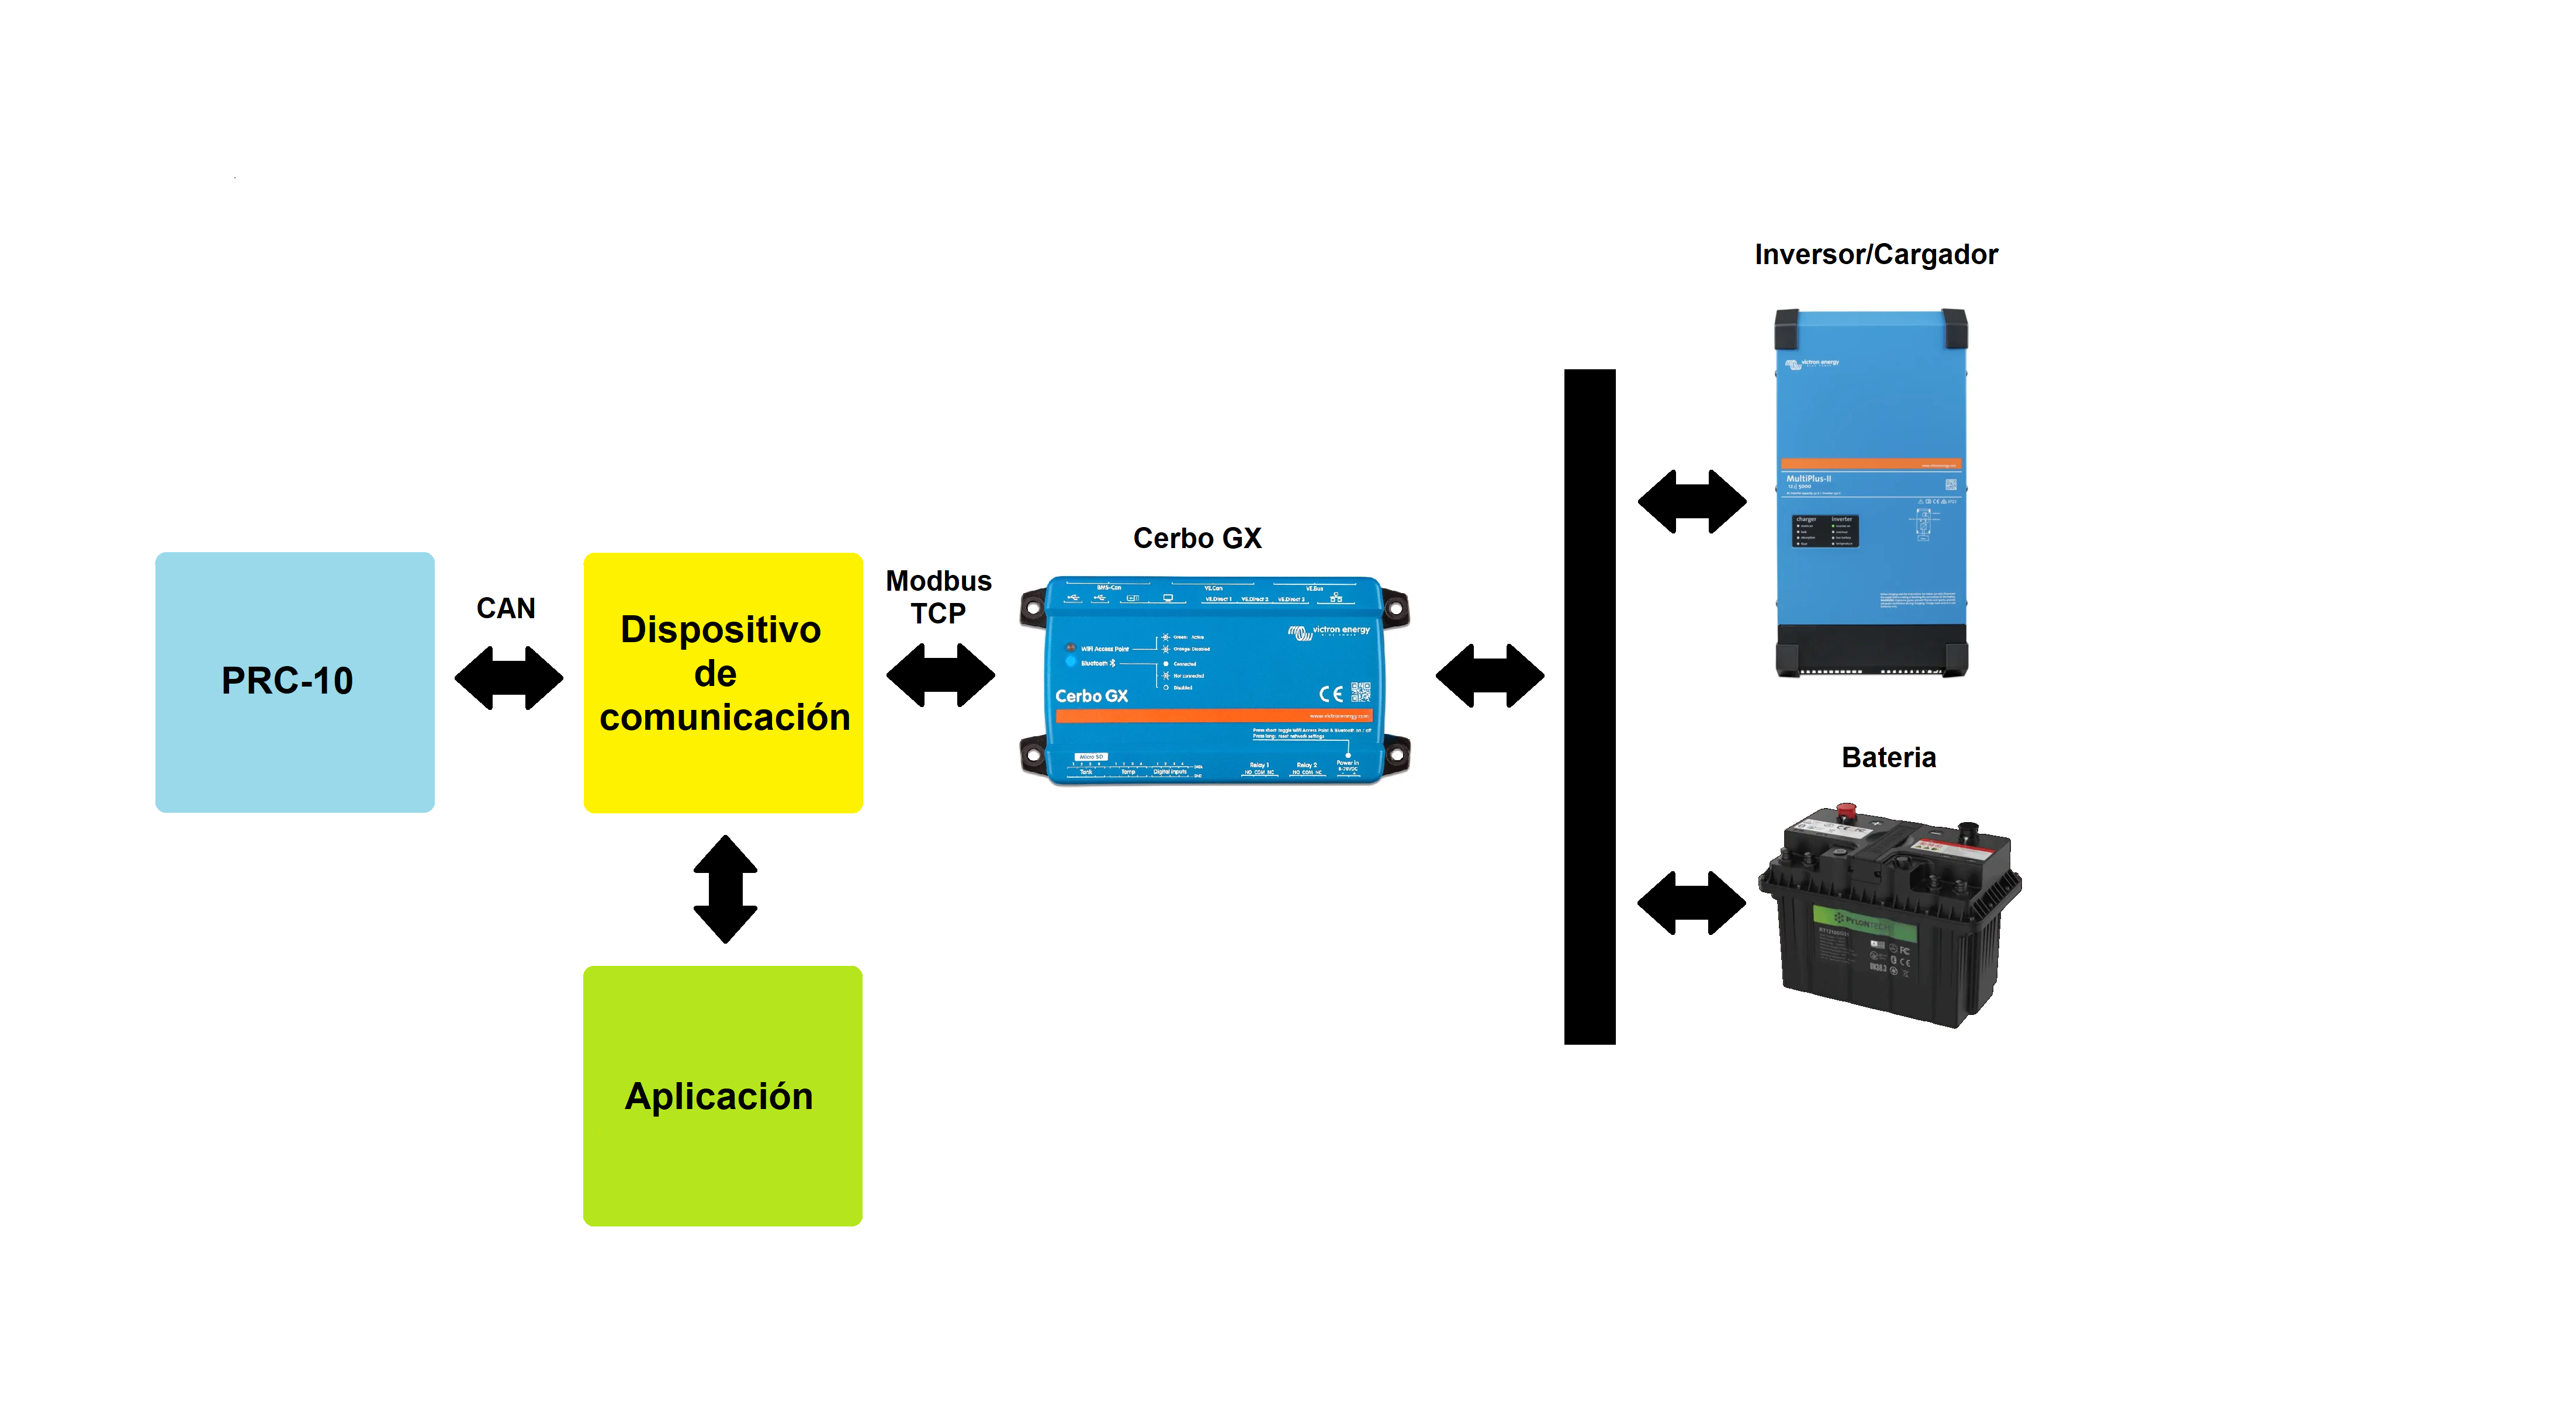
\includegraphics[width=\textwidth]{./Figuras/esquema.png}
\caption{Diagrama en bloques del sistema.}
\label{fig:esquema}
\end{figure}

Para la comunicación con el Cerbo GX, Victron Energy proporciona (en su sitio web) guías y documentación técnica que permiten implementar el monitoreo y control de sus dispositivos mediante el protocolo Modbus TCP. Por otra parte, la comunicación con la PRC10 deberá ser por protocolo CAN.

Para el control de la red de domótica, Enertik dispone de una pantalla que cumple la función de HMI. En relación con esto, se deberá desarrollar una aplicación que replique, en la medida de lo posible, todas las funcionalidades de dicha pantalla, así como también permita monitorear y controlar los equipos conectados a la red Victron.

Con este desarrollo se busca brindar a los clientes una alternativa adicional para gestionar y controlar los sistemas integrados en el motorhome.

Este dispositivo de comunicación no existe a la fecha de elaboración de este documento, por lo que deberá ser desarrollado en su totalidad. Esto incluye el diseño del PCB, el desarrollo del firmware para el microcontrolador (ESP32) y la creación de la aplicación mencionada anteriormente.

Este equipo está previsto para convertirse en un producto comercial, por lo que se solicitará la firma de acuerdos de confidencialidad a todas las personas involucradas en su desarrollo (alumno responsable, director, jurados, etc.).

\section{2. Identificación y análisis de los interesados}
\label{sec:interesados}

\begin{table}[ht]
%\caption{Identificación de los interesados}
%\label{tab:interesados}
\begin{tabularx}{\linewidth}{@{}|l|X|X|l|@{}}
\hline
\rowcolor[HTML]{C0C0C0} 
Rol           & Nombre y Apellido 		& Organización 	& Puesto 	\\ \hline
Cliente       & \clientename  		  &\empclientename	& Director Enertik    \\ \hline
Responsable   & \authorname     		  & Enertik Argentina - FIUBA        	& Alumno 	\\ \hline
Orientador    & \supname     		 & \pertesupname 	& Director Trabajo final \\ \hline
Usuario final & Fabricantes de motorhomes & Varios    	& -       	\\ \hline
\end{tabularx}
\end{table}

\begin{itemize}
	\item Cliente: evaluará el cumplimiento de objetivos.
	\item Orientador: participará continuamente durante la ejecución del proyecto, guiando y aconsejando sobre el uso de las distintas herramientas.
	\item Usuarios finales: fabricantes de motorhomes para implementarlos en su red de domótica interna.
\end{itemize}


\section{3. Propósito del proyecto}
\label{sec:proposito}

Desarrollar un dispositivo de comunicación que permita la integración de equipos de la marca Victron Energy a la red de domótica provista por Enertik, junto con una aplicación que ofrezca al usuario final una alternativa adicional para el control y monitoreo de los distintos sistemas integrados en el motorhome.

\section{4. Alcance del proyecto}
\label{sec:alcance}

El presente proyecto incluye:

\begin{itemize}
	\item Desarrollo del firmware para el microcontrolador (ESP32).
	\item Diseño de la placa de circuito impreso (PCB).
	\item Generación de lista de componentes para montaje (BOM).
	\item Desarrollo de una aplicación que permita el control tanto de la red Victron como de la red de domótica.
	\item Pruebas funcionales de integración entre la PRC10 y el Cerbo GX.	
\end{itemize}

El proyecto no incluye:
\begin{itemize}
	\item Diseño del gabinete o carcasa para el PCB.
	\item Redacción de manuales de uso o documentación para el usuario final.	
\end{itemize}

\section{5. Supuestos del proyecto}
\label{sec:supuestos}

Para el desarrollo del presente proyecto se supone que: 

\begin{itemize}
	\item Se dispondrá, en tiempo y forma, de las materias primas necesarias para el desarrollo del hardware.
	\item Se contará con acceso a herramientas de diseño electrónico (como Altium Designer) y entornos de desarrollo (IDE, compiladores, etc.).
	\item La empresa Enertik aportará los equipos de Victron Energy requeridos para la realización de los ensayos.
	\item Enertik pondrá a disposición el módulo PRC10, así como los demás dispositivos necesarios para las pruebas.
	\item La documentación técnica provista en el sitio web de Victron Energy será suficiente y adecuada para establecer la red de comunicación mediante Modbus TCP.
	\item En caso de requerir orientación o asesoramiento, se contará con el apoyo del director del proyecto, así como también del personal de Enertik con experiencia en redes Victron.
	
\end{itemize}

\section{6. Requerimientos}
\label{sec:requerimientos}

\begin{enumerate}
	\item Requerimientos en el dispositivo:
		\begin{enumerate}
			\item Debe establecer comunicación con el Cerbo GX utilizando el protocolo Modbus TCP sobre Ethernet o Wi-Fi.
			\item Debe comunicarse con el módulo PRC10 a través del protocolo CAN.
			\item Debe generar una red Wi-Fi en modo Access Point con SSID configurable.
			\item La frecuencia de actualización de datos debe ser de aproximadamente veinte segundos.			
		\end{enumerate}
	\item Requerimientos en la aplicación:
		\begin{enumerate}
			\item Debe conectarse al sistema embebido mediante la red Wi-Fi generada por este.
			\item Debe mostrar en tiempo real el estado de las variables monitoreadas.
			\item Debe permitir el envío de comandos para el control de los dispositivos de domótica.
			\item Debe ser accesible desde dispositivos con sistema operativo Android.
			\item Puede incluir la funcionalidad de autenticación de usuario para acceso a los controles del sistema.
		\end{enumerate}
	\item Requerimientos generales:
		\begin{enumerate}
			\item El sistema debe operar de forma autónoma, sin requerir conexión a Internet.
			\item El equipo debe alimentarse a través de la red física de 12 VDC (+12, GND, CAN H, CAN L) utilizada por los demás dispositivos.
		\end{enumerate}
\end{enumerate}

\section{7. Historias de usuarios (\textit{Product backlog})}
\label{sec:backlog}

Para definir los story points se utilizará la serie de Fibonacci.

Por otra parte, la tabla de pesos a utilizar será:
\begin{enumerate}
\item Dificultad en el trabajo a realizar:
	\begin{itemize}
		\item Baja: peso 1.
		\item Media: peso 3.
		\item Alta: peso 5.
	\end{itemize}

\item Complejidad en el trabajo a realizar:
	\begin{itemize}
		\item Baja: peso 1.
		\item Media: peso 4.
		\item Alta: peso 7.
	\end{itemize}

\item Incertidumbre en el trabajo a realizar:
	\begin{itemize}
		\item Baja: peso 2.
		\item Media: peso 3.
		\item Alta: peso 5.
	\end{itemize}
\end{enumerate}

Historias de usuario:
\begin{enumerate}
	\item Como usuario final, quiero conectarme desde mi teléfono a la red Wi-Fi del dispositivo para poder visualizar y controlar los sistemas del motorhome.
		\begin{itemize}
			\item Dificultad: media.
			\item Complejidad: media.
			\item Incertidumbre: alto.
			\item Story point: 13.
	\end{itemize}
	\item Como usuario final, quiero encender y apagar dispositivos de la red de domótica desde la aplicación para controlar el ambiente del motorhome.
		\begin{itemize}
			\item Dificultad: bajo.
			\item Complejidad: media.
			\item Incertidumbre: bajo.
			\item Story point: 8.
	\end{itemize}
	\item Como desarrollador, quiero que el dispositivo lea datos del Cerbo GX usando Modbus TCP para integrarlos al sistema de monitoreo.
		\begin{itemize}
			\item Dificultad: alto.
			\item Complejidad: media.
			\item Incertidumbre: media.
			\item Story point: 13.
	\end{itemize}
	\item Como instalador, quiero que el dispositivo se alimente desde la red física existente (+12, GND, CAN H, CAN L) para facilitar la integración en el motorhome.
		\begin{itemize}
			\item Dificultad: media.
			\item Complejidad: media.
			\item Incertidumbre: bajo.
			\item Story point: 8.
	\end{itemize}
	\item Como desarrollador, quiero que el dispositivo se comunique con la PRC10 mediante CAN para poder integrar el nuevo sistema a la red de domótica.
		\begin{itemize}
			\item Dificultad: alta.
			\item Complejidad: media.
			\item Incertidumbre: alta.
			\item Story point: 13.
	\end{itemize}
\end{enumerate}

\section{8. Entregables principales del proyecto}
\label{sec:entregables}
Los entregables del proyecto son:

\begin{itemize}
	\item Prototipo funcional del dispositivo de comunicación.
	\item Diagrama esquemático del circuito.
	\item Código fuente del firmware.
	\item Código fuente de la aplicación móvil
	\item Lista de componentes para montaje (BOM).
	\item Archivos gerber para fabricación de PCB.
	\item Instalador de la aplicación (en caso de ser implementado).
	\item Memoria final de trabajo.
\end{itemize}

\section{9. Desglose del trabajo en tareas}
\label{sec:wbs}


\begin{enumerate}
\item Análisis inicial (30 h)
	\begin{enumerate}
	\item Revisión de la documentación de microcontrolador ESP32 (5 h).
	\item Revisión de la documentación de Victron Energy y Modbus TCP (20 h).
	\item Preparación del entorno de desarrollo IDE (5 h).
	\end{enumerate}
\item Desarrollo de hardware (233 h)
	\begin{enumerate}
	\item Configuración de periféricos sobre el ESP32: pines, timers, puertos, RTOS (10 h).
	\item Implementación de la red Wi-FI como Acess Point: configuración y manejo de conexión (10 h).
	\item Desarrollo de comunicación con el módulo PRC10
		\begin{enumerate}
		\item Protocolo CAN: implementación con MCP2551 (10 h).
		\item Desarrollo del módulo transceiver (10 h).
		\item Incorporación de los comandos utilizados en la PRC10 (10 h).
		\item Modificación del firmware de la PRC10 (20 h).
		\item Ensayos de comunicación entre ESP32 y PRC10 (20 h).
		\end{enumerate}	
	\item Desarrollo de comunicación con el módulo Cerbo GX
		\begin{enumerate}
		\item Desarrollo de la biblioteca con la información de todos los dispositivos de Victron Energy (25 h).
		\item Modbus TCP: implementación por Wi-Fi (30 h).
		\item Modbus TCP: implementación por Ethernet con W5100 (30 h).		
		\item Incorporación de los comandos y funciones para operar con los registros Modbus (30 h).
		\item Análisis y comporativa entre implementación Wi-Fi y Ethernet (8 h).
		\item Ensayos de comunicación entre ESP32 y Cerbo GX (20 h).
		\end{enumerate}		
	\end{enumerate}
\item Desarrollo de la aplicación (260 h)
	\begin{enumerate}
		\item Análisis y evaluación: aplicación embebida y aplicación nativa para Android (10 h).
		\item Diseño de esquemas para interfaces gráficas (15 h).
		\item Desarrollo de aplicación embebida
		\begin{enumerate}
			\item Desarrollo de estructura en HTML (25 h).
			\item Estilos visuales con CSS (25 h).
			\item Manejo de peticiones y funciones con Javascript - Typescript (35 h).
			\item Conversión de formato y carga de archivos al ESP32 (15 h).
			\item Ensayos con distintos navegadores y dispositivos (15 h).
		\end{enumerate}
		\item Desarrollo de la aplicación nativa para Android
		\begin{enumerate}
			\item Creación y configuración del proyecto en Angular (10 h).
			\item Desarrollo de componentes y vistas (HTML - CSS - Javascript) (30 h).
			\item Implementación de la comunicación con el ESP32 por WebSocket (15 h).
			\item Configuración en Android Studio para generación de APK (10 h).
			\item Ensayos en distintos dispositivos móviles (15 h).
		\end{enumerate}
		\item Desarrollo de backend
		\begin{enumerate}
			\item Definición de endpoints y estructura de API (REST / WebSocket) (5 h).
			\item Implementación del servidor HTTP en ESP32 (10 h).
			\item Programación del canal WebSocket para datos en tiempo real (10 h).
			\item Gestión de solicitudes de la aplicación (10 h).
			\item Pruebas de carga y depuración del backend (5 h).
		\end{enumerate}	
	\end{enumerate}
\item Desarrollo de PCB (78 h)
	\begin{enumerate}
		\item Diseño de prototipo experimental (25 h).
		\item Desarrollo de PCB con Altium Designer (35 h).
		\item Fabricación: generación de archivos gerber e inicio de tramite de fabricación (10 h).
		\item Elaboración del diagrama esquemático del circuito y confección de la lista de materiales (BOM) para montaje (8 h).
	\end{enumerate}
\item Redacción de informe final para maestría (70 h)
	\begin{enumerate}
		\item Redacción del informe de avance (10 h).
		\item Redacción del informe final del proyecto (40 h).
		\item Elaboración de la presentación (20 h).
	\end{enumerate}
\end{enumerate}

Cantidad total de horas: 671 h.

\section{10. Diagrama de Activity On Node}
\label{sec:AoN}

La figura \ref{fig:aongeneral} muestra el diagrama Activity on Node general del proyecto, junto con el tiempo que demandará cada tarea (expresado en horas).

Se puede observar que el camino crítico (representado por el trayecto en rojo) tomará unas 411 horas de trabajo.

\begin{figure}[htpb]
\centering 
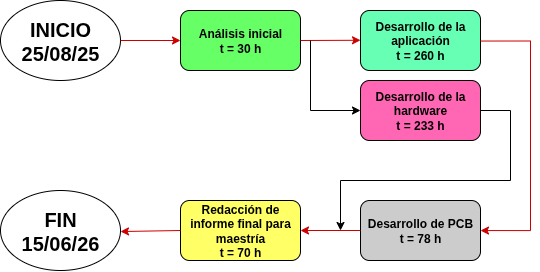
\includegraphics[width=.8\textwidth]{./Figuras/aon_general.png}
\caption{Diagrama de \textit{Activity on Node general}.}
\label{fig:aongeneral}
\end{figure}

A continuación, se mostrarán los diagramas Activity on Node que representan a las distintas subtareas, junto con el tiempo que demandarán cada una de ellas (expresado en horas). El camino crítico quedará representado por el trayecto de color rojo.

\begin{itemize}
			\item La figura \ref{fig:tareas_1} muestra las subtareas 1.
			\item La figura \ref{fig:tareas_2} muestra las subtareas 2.
			\item La figura \ref{fig:tareas_3} muestra las subtareas 3.
			\item La figura \ref{fig:tareas_4} muestra las subtareas 4.
			\item La figura \ref{fig:tareas_5} muestra las subtareas 5.
	\end{itemize}

\begin{figure}[H]
\centering
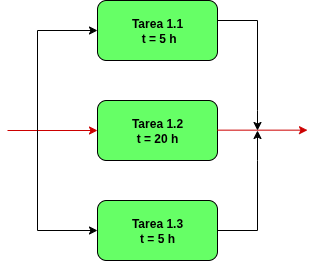
\includegraphics[scale=0.6]{./Figuras/tareas_1.png}
\caption{Activity on Node (tareas 1).}
\label{fig:tareas_1}
\end{figure}

\begin{figure}[H]
\centering
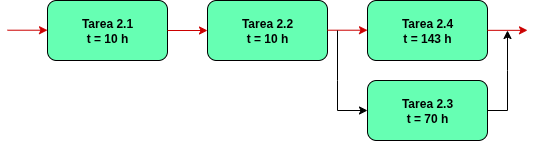
\includegraphics[scale=0.6]{./Figuras/tareas_2.png}
\caption{Activity on Node (tareas 2).}
\label{fig:tareas_2}
\end{figure}

\begin{figure}[H]
\centering
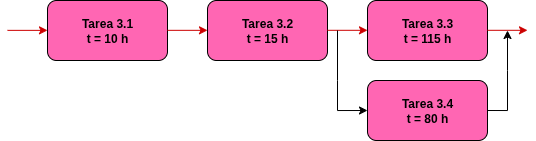
\includegraphics[scale=0.6]{./Figuras/tareas_3.png}
\caption{Activity on Node (tareas 3).}
\label{fig:tareas_3}
\end{figure}


\begin{figure}[H]
\centering
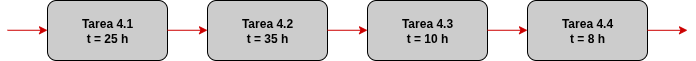
\includegraphics[scale=0.6]{./Figuras/tareas_4.png}
\caption{Activity on Node (tareas 4).}
\label{fig:tareas_4}
\end{figure}

\begin{figure}[H]
\centering
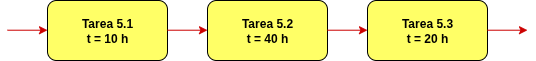
\includegraphics[scale=0.6]{./Figuras/tareas_5.png}
\caption{Activity on Node (tareas 5).}
\label{fig:tareas_5}
\end{figure}

\section{11. Diagrama de Gantt}
\label{sec:gantt}

Las figuras \ref{fig:gantt1} y \ref{fig:gantt2} muestran el diagrama de Gantt del proyecto. Cada una de las tareas se ven reflejadas en la tabla que muestra la figura \ref{fig:wbs}.

\begin{figure}[H]
\centering
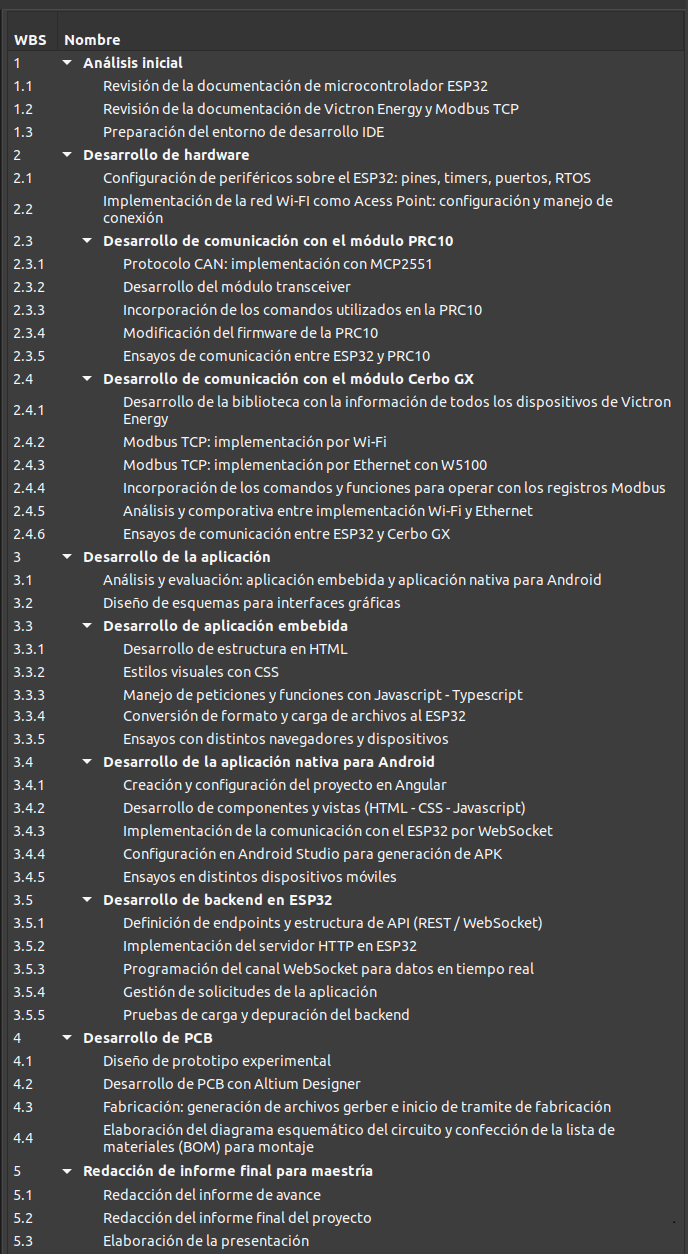
\includegraphics[scale=0.34]{./Figuras/tareas2.png}
\caption{Lista de tareas.}
\label{fig:wbs}
\end{figure}

\begin{landscape}
\begin{figure}
\centering 
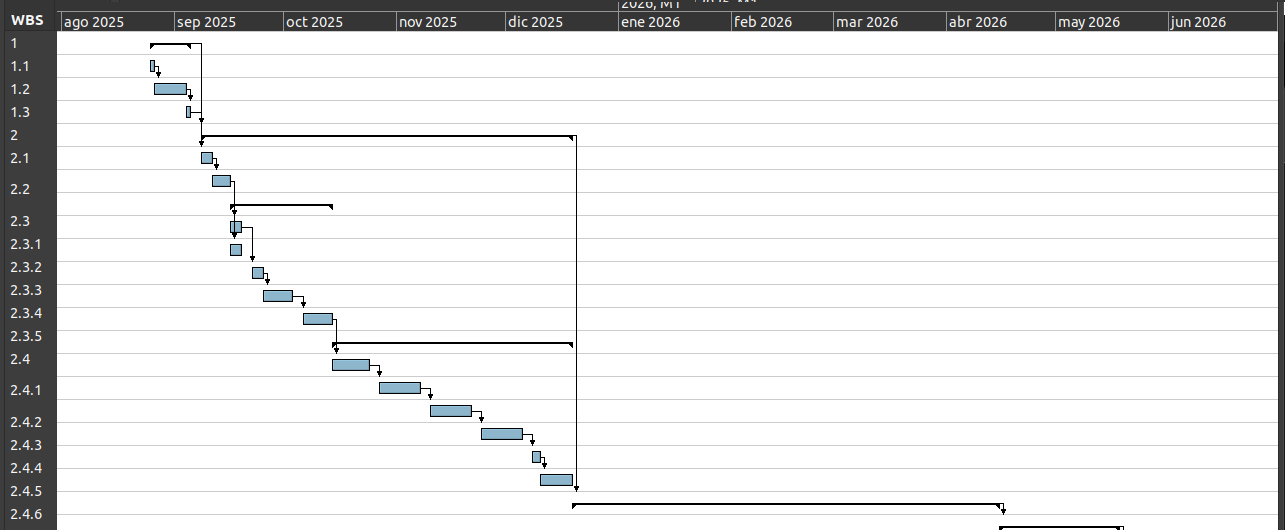
\includegraphics[scale=0.7]{./Figuras/gantt_1.png}
\caption{Diagrama de Gantt (tareas 1 y 2).}
\label{fig:gantt1}
\end{figure}

\end{landscape}

\begin{landscape}
\begin{figure}
\centering 
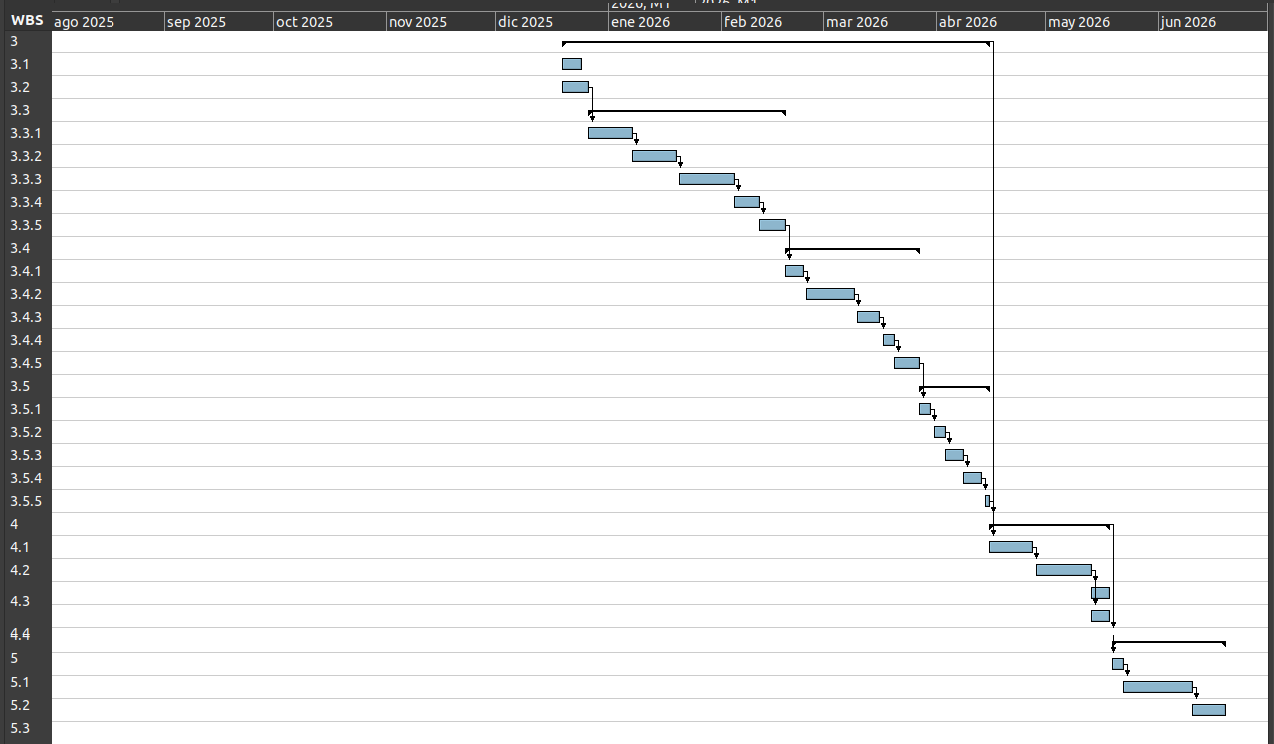
\includegraphics[scale=0.7]{./Figuras/gantt_2.png}
\caption{Diagrama de Gantt (tareas 3, 4 y 5).}
\label{fig:gantt2}
\end{figure}

\end{landscape}





\section{12. Presupuesto detallado del proyecto}
\label{sec:presupuesto}

A continuación ,se detallará el presupuesto del proyecto. La cotización se encuentra expresada en dólares estadounidenses (USD) y, al día de la fecha, se considera una equivalencia de 1 USD=\$1300 ARS.

\begin{table}[htpb]
\centering
\begin{tabularx}{\linewidth}{@{}|X|c|r|r|@{}}
\hline
\rowcolor[HTML]{C0C0C0} 
\multicolumn{4}{|c|}{\cellcolor[HTML]{C0C0C0}COSTOS DIRECTOS} \\ \hline
\rowcolor[HTML]{C0C0C0} 
Descripción &
  \multicolumn{1}{c|}{\cellcolor[HTML]{C0C0C0}Cantidad} &
  \multicolumn{1}{c|}{\cellcolor[HTML]{C0C0C0}Valor unitario} &
  \multicolumn{1}{c|}{\cellcolor[HTML]{C0C0C0}Valor total} \\ \hline
\multicolumn{1}{|l|}{Horas de trabajo} &671
   &\multicolumn{1}{c|}{US\$ 15}
   &\multicolumn{1}{c|}{US\$ 10.065}
   \\ \hline
\multicolumn{1}{|l|}{Módulo ESP32} &1
   &\multicolumn{1}{c|}{US\$ 10}
   &\multicolumn{1}{c|}{US\$ 10}
   \\ \hline
\multicolumn{1}{|l|}{Módulo W5100} &1
   &\multicolumn{1}{c|}{US\$ 6}
   &\multicolumn{1}{c|}{US\$ 6}
   \\ \hline
\multicolumn{1}{|l|}{Módulo MCP2551} &1
   &\multicolumn{1}{c|}{US\$ 5}
   &\multicolumn{1}{c|}{US\$ 5}
   \\ \hline
\multicolumn{1}{|l|}{PCB experimental para prototipo} &1
   &\multicolumn{1}{c|}{US\$ 1}
   &\multicolumn{1}{c|}{US\$ 1}
   \\ \hline
\multicolumn{1}{|l|}{PCB definitivo comercial} &1
   &\multicolumn{1}{c|}{US\$ 35}
   &\multicolumn{1}{c|}{US\$ 35}
   \\ \hline
\multicolumn{1}{|l|}{Componentes pasivos varios} &1
   &\multicolumn{1}{c|}{US\$ 20}
   &\multicolumn{1}{c|}{US\$ 20}
   \\ \hline
\multicolumn{3}{|c|}{SUBTOTAL} &
  \multicolumn{1}{c|}{US\$ 10.142} \\ \hline
\rowcolor[HTML]{C0C0C0} 
\multicolumn{4}{|c|}{\cellcolor[HTML]{C0C0C0}COSTOS INDIRECTOS} \\ \hline
\rowcolor[HTML]{C0C0C0} 
Descripción &
  \multicolumn{1}{c|}{\cellcolor[HTML]{C0C0C0}Cantidad} &
  \multicolumn{1}{c|}{\cellcolor[HTML]{C0C0C0}Valor unitario} &
  \multicolumn{1}{c|}{\cellcolor[HTML]{C0C0C0}Valor total} \\ \hline
\multicolumn{1}{|l|}{50 \% de los costos directos } &\multicolumn{1}{c|}{1}
   &\multicolumn{1}{c|}{US\$ 5.071}
   &\multicolumn{1}{c|}{US\$ 5.071}
   \\ \hline
\multicolumn{3}{|c|}{SUBTOTAL} &
  \multicolumn{1}{c|}{US\$ 5.071} \\ \hline
\rowcolor[HTML]{C0C0C0}
\multicolumn{3}{|c|}{TOTAL} & \multicolumn{1}{c|}{US\$ 15.213}
   \\ \hline
\end{tabularx}%
\end{table}

\section{13. Gestión de riesgos}
\label{sec:riesgos}

a) Identificación de los riesgos y estimación de sus consecuencias:

Riesgo 1: dificultad para conseguir los elementos necesarios para el desarrollo del hardware.
\begin{itemize}
	\item Severidad (S): 9.\\
	No contar con estos elementos en tiempo y forma ocasionará un retraso en el desarrollo del proyecto.
	\item Probabilidad de ocurrencia (O): 2.\\
	Los elementos elegidos durante la planificación son bastantes accesibles en Argentina (muchos proveedores los comercializan).
\end{itemize}

Riesgo 2: falta de información o claridad proporcionada en la web de Victron Energy.
\begin{itemize}
	\item Severidad (S): 8.\\
	Cualquier faltante de información dificultará el desarrollo del proyecto.
	\item Probabilidad de ocurrencia (O): 4.\\
	Victron Energy pone a disposición un amplio abanico de guías y manuales para este tipo de desarrollo.
\end{itemize}      

Riesgo 3: incertidumbre respecto al alcance del control de los equipos mediante el protocolo Modbus TCP
\begin{itemize}
	\item Severidad (S): 7.\\
	Si la cantidad de variables disponibles para controlar o monitorear resulta limitada, la funcionalidad del dispositivo quedará restringida y reducirá su integración con la red de domótica.
	\item Probabilidad de ocurrencia (O): 8.\\
	Los registros accesibles a través de Modbus TCP son finitos y es probable que varios parámetros relevantes no estén disponibles, lo que afectará el alcance del monitoreo.
\end{itemize}  

Riesgo 4: problemas en la comunicación entre la aplicación y el ESP32.
\begin{itemize}
	\item Severidad (S): 9.\\
	Si la comunicación falla, pueden producirse lecturas erróneas de datos o la ejecución incorrecta de comandos, lo que afectaría el funcionamiento del dispositivo y la red de domótica.
	\item Probabilidad de ocurrencia (O): 7.\\
	 Existe la posibilidad de saturación del sistema, especialmente si se intenta mantener una comunicación en tiempo real con alto volumen de mensajes.
\end{itemize}

Riesgo 5: imposibilidad de adaptar el firmware del módulo PRC10.
\begin{itemize}
	\item Severidad (S): 10.\\
	Si no es posible realizar las modificaciones necesarias en el firmware, se impediría la integración de los equipos Victron con la red de domótica.
	\item Probabilidad de ocurrencia (O): 2.\\
	 El firmware es provisto por Enertik, por lo que se tendrá acceso a su código fuente.
\end{itemize}

b) Tabla de gestión de riesgos      (El RPN se calcula como RPN=SxO):

\begin{table}[htpb]
\centering
\begin{tabularx}{\linewidth}{@{}|X|c|c|c|c|c|c|@{}}
\hline
\rowcolor[HTML]{C0C0C0} 
Riesgo & S & O & RPN & S* & O* & RPN* \\ \hline
Dificultad en la obteción de componentes       &  9 & 2  &  18   &    &    &      \\ \hline
Falta de información por parte de Victro Energy       &  8 &  4 &  32   &    &    &      \\ \hline
Incertidumbre en el alcance de control de los equipos       & 7  & 8  & 56    &   7 & 6   & 42     \\ \hline
Problemas en la comunicación entre aplicación y ESP32       &  9 & 7  & 63    &  8  & 6   & 48     \\ \hline
Imposibilidad de adaptar el firmware del módulo PRC10       & 10  & 2  & 20    &    &    &      \\ \hline
\end{tabularx}%
\end{table}

Criterio adoptado: 

Se tomarán medidas de mitigación en los riesgos cuyos números de RPN sean mayores a 50.

c) Plan de mitigación de los riesgos que originalmente excedían el RPN máximo establecido:
 
Riesgo 3: se realizará un relevamiento completo de la documentación de Victron Energy y, en caso de detectar alguna limitación, se priorizarán los parámetros mas relevantes para el usuario final.
 
  \begin{itemize}
	\item Severidad (S*): 7.\\
          La severidad no variará.
	\item Probabilidad de ocurrencia (O*): 6.\\
          Una investigación anticipada y la definición clara de qué variables serán controladas reducirán la incertidumbre y la probabilidad de que este riesgo se manifieste.
	\end{itemize}
	
Riesgo 4: se definirá una tasa de intercambio de datos moderada y estable, evitando la saturación del sistema sin comprometer las funciones esenciales de control y monitoreo.
 
  \begin{itemize}
	\item Severidad (S*): 8.\\
          Una menor carga de datos reducirá el impacto de fallas de comunicación.
	\item Probabilidad de ocurrencia (O*): 6.\\
          La probabilidad de ocurrencia no variará.
	\end{itemize}


\section{14. Gestión de la calidad}
\label{sec:calidad}

\begin{itemize} 
\item 1.1 Debe establecer comunicación con el Cerbo GX utilizando el protocolo Modbus TCP sobre Ethernet o Wi-Fi.

\begin{itemize}
	\item Verificación: se realizarán ensayos de comunicación en los que el ESP32 enviará comandos de lectura y escritura a los registros del Cerbo GX a través de cable Ethernet y/o Wi-Fi.
	\item Validación: el cliente validará la comunicación ejecutando operaciones de monitoreo y control sobre los equipos de Victron Energy en condiciones normales de uso. 
\end{itemize}

\item 1.2 Debe comunicarse con el módulo PRC10 a través del protocolo CAN.

\begin{itemize}
	\item Verificación: se realizarán pruebas de comunicación en las que el ESP32 enviará y recibirá mensajes CAN hacia y desde el módulo PRC10, verificando la correcta interpretación de comandos y la estabilidad del enlace.
	\item Validación: el cliente validará el funcionamiento probando operaciones de control y monitoreo de la red de domótica mediante el PRC10, confirmando que la comunicación cumple con lo especificado.
\end{itemize}

\item 1.3 Debe generar una red Wi-Fi en modo Access Point con SSID configurable.

\begin{itemize}
	\item Verificación: se realizarán pruebas para verificar que el ESP32 pueda crear una red Wi‑Fi en modo Access Point, comprobar la visibilidad del SSID y la posibilidad de modificarlo desde la configuración del dispositivo.
	\item Validación: el cliente validará el funcionamiento conectándose a la red creada, cambiando el SSID y confirmando que el acceso y la comunicación se mantienen correctos después de cada modificación.
\end{itemize}

\item 2.1 Debe conectarse al sistema embebido mediante la red Wi-Fi generada por este.
\begin{itemize}
	\item Verificación: se realizarán pruebas conectando distintos dispositivos móviles (Android) a la red Wi‑Fi creada por el ESP32. Se verificará que la aplicación pueda establecer conexión con el sistema embebido, enviar solicitudes y recibir datos sin pérdida de información.
	\item  Validación: el cliente probará la conexión desde diferentes dispositivos y confirmará que la aplicación se conecta correctamente y mantiene la comunicación estable con el sistema embebido.
\end{itemize}

\item 2.2 Debe mostrar en tiempo real el estado de las variables monitoreadas.
\begin{itemize}
	\item Verificación: se programará un test en el ESP32 que simule el envío de datos de todos los dispositivos a la aplicación. Se comprobará que los valores reflejados en la aplicación coincidan con los generados por el microcontrolador, respetando una latencia máxima establecida.
	\item Validación: el cliente verificará, en condiciones de uso real, que la aplicación muestre los datos actualizados sin retrasos significativos y confirmará que la frecuencia de actualización cumple con lo requerido.
\end{itemize}

\item 2.3 Debe permitir el envío de comandos para el control de los dispositivos de domótica.
\begin{itemize}
	\item Verificación: se establecerán funciones de registro (LOG) en el ESP32 que muestren un mensaje en la PC cada vez que se reciba un comando desde la aplicación, indicando qué acción ejecutará como respuesta.
	\item Validación: el cliente probará la aplicación enviando comandos en condiciones de uso real y confirmará que los dispositivos respondan de manera inmediata y conforme a lo solicitado.
\end{itemize}

\item 3.2 El equipo debe alimentarse a través de la red física de 12 VDC (+12, GND, CAN H, CAN L) utilizada por los demás dispositivos.
\begin{itemize}
	\item Verificación: se realizarán pruebas de alimentación conectando el equipo a la red física de 12 VDC y verificando su correcto funcionamiento sin interrupciones ni daños.
	\item Validación: el cliente confirmará que el equipo opera adecuadamente cuando se alimenta desde la red física compartida con los demás dispositivos.
\end{itemize}

\end{itemize}


\section{15. Procesos de cierre}    
\label{sec:cierre}
\begin{enumerate}
\item Cumplimiento del plan de trabajo.
	\begin{itemize}
	\item Se tomará en cuenta el tiempo que realmente fue necesario emplear para llevar a cabo cada una de las tareas, y se lo comparará con lo planificado originalmente.
	\item Responsable: Matías Nahuel Rodriguez.
	\end{itemize}
\item Identificación de las técnicas y procedimientos empleados.
	\begin{itemize}
	\item Durante el desarrollo del proyecto, se documentarán de forma sistemática todos los procedimientos y técnicas aplicados, independientemente de si los resultados fueron satisfactorios o no. Esta documentación permitirá registrar el proceso completo seguido para cumplir con los requerimientos. Además, se utilizará GitHub como herramienta de control de versiones para dejar constancia del desarrollo del producto final.
	\item Responsable: Matías Nahuel Rodriguez.
	\end{itemize}
\item Acto de agradecimientos.
	\begin{itemize}
	\item La defensa del proyecto se realizará una vez este haya culminado. Aquí se agradecerá a las distintas personas que colaboraron durante la ejecución del proyecto, así como también al personal que conforma a la CEIoT.
	\item Responsable: Matías Nahuel Rodriguez.
	\end{itemize}
\end{enumerate}


\end{document}